% ══════════════════════════════════════════════════════════════════════════════
%  Presentation: structure of the report
%  "From Optimal Control to Diffusion Policy" — Group Project TN2
%  Build from the report/ folder so images/ paths resolve:
%      latexmk -pdf presentation.tex      (or pdflatex presentation.tex)
% ══════════════════════════════════════════════════════════════════════════════
\documentclass[aspectratio=169,11pt]{beamer}

% ── Theme ─────────────────────────────────────────────────────────────────────
\usetheme{metropolis}
\metroset{block=fill, numbering=fraction, progressbar=frametitle}

\usepackage{amsmath,amssymb}
\usepackage{graphicx}
\usepackage{booktabs}
\usepackage{xcolor}
\usepackage{animate}   % inline GIF animation (\animategraphics) — plays in Acrobat
\usepackage{media9}    % embedded video (\includemedia) — plays in Acrobat

\definecolor{bcblue}{rgb}{0.10,0.35,0.65}
\definecolor{dpred}{rgb}{0.70,0.20,0.15}
\newcommand{\BC}{\textcolor{bcblue}{\textbf{BC}}}
\newcommand{\DP}{\textcolor{dpred}{\textbf{Diffusion}}}

% ── Title ─────────────────────────────────────────────────────────────────────
\title{From Optimal Control to Diffusion Policy}
\subtitle{Behavioural Cloning vs.\ Diffusion Policy on Double-Pendulum Swing-Up \& Cube Stacking}
\author{Group Project TN2}
\date{\today}

\begin{document}

\maketitle

% ── Outline ───────────────────────────────────────────────────────────────────
\begin{frame}{Outline}
  \tableofcontents
\end{frame}

% ══════════════════════════════════════════════════════════════════════════════
\section{Introduction}

\begin{frame}{Goal of the project}
  \begin{block}{Question}
    Compare two \alert{imitation-learning} control methods on the same data.
  \end{block}
  \begin{columns}[T]
    \begin{column}{0.5\textwidth}
      \textbf{\BC{} (baseline)}\\
      Regress the expert action directly from the state — a single deterministic map.
    \end{column}
    \begin{column}{0.5\textwidth}
      \textbf{\DP{} Policy}\\
      Generate an action \emph{chunk} from noise by iterative denoising, conditioned on the state.
    \end{column}
  \end{columns}
  \vfill
  \textbf{Two tasks}
  \begin{itemize}
    \item Double-pendulum \alert{swing-up} (small, fast, unstable balance task)
    \item Robotic \alert{cube stacking} — Stack (2 cubes) and StackThree (3 cubes)
  \end{itemize}
  Same demonstrations per task $\Rightarrow$ the comparison reflects the \emph{method}, not the data.
\end{frame}

% ══════════════════════════════════════════════════════════════════════════════
\section{Part I — Double-Pendulum Swing-Up}

\begin{frame}{Part I — roadmap}
  \begin{enumerate}
    \item \textbf{BC model} — network \& training
    \item \textbf{Diffusion background} — forward / reverse process
    \item \textbf{Generating the expert dataset} — TrajOpt $\rightarrow$ TVLQR $\rightarrow$ rollout
    \item \textbf{Diffusion Policy model} — conditioning, network, control tricks
    \item \textbf{Comparison} — metrics, robustness, ablations
  \end{enumerate}
\end{frame}

\begin{frame}{1. Behavioural Cloning -  Network Architecture}
  \begin{columns}[T]
    \begin{column}{0.33\textwidth}
      \begin{itemize}
        \item Input: feature transform $\phi(s_t)\in\mathbb{R}^{6}$
        \item 4 hidden fully-connected layers, $\tanh$, dropout with probability $0.2$
        \item Output $16 \to$ reshaped to $8\times2$ torques
      \end{itemize}
    \end{column}
    \begin{column}{0.66\textwidth}
      \centering
      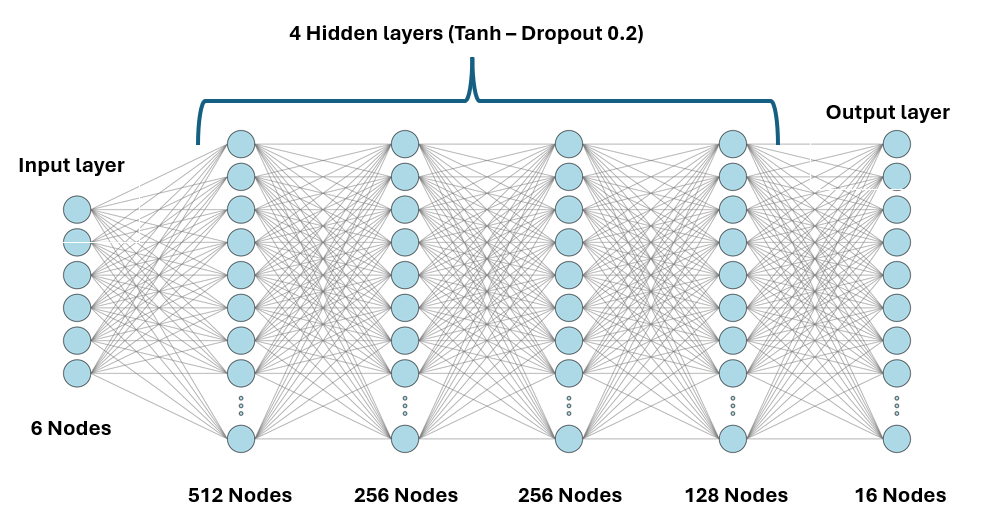
\includegraphics[width=\linewidth]{images/part1/neural network.png}\\
      {\scriptsize BC Model architecture.}
    \end{column}
  \end{columns}
\end{frame}

\begin{frame}{2. BC - Training}
  \begin{columns}[T]
    \begin{column}{0.55\textwidth}
      Learn $\pi = (a_{t:t+7}\mid s_t)$ — an 8-step action chunk.
      \begin{itemize}
      \item Wrap-safe angular features
          $\phi=[\sin q_1,\cos q_1,\dots,\tilde{\dot {q}}_2]\in\mathbb{R}^{6}$
        \item Min--max normalise to $[-1,1]$ actions and velocities (stats saved)
        \item $90/10$ train/val
        \item MSE loss, Adam $10^{-3}$, early stop (no overfit)
        \item 512 batch size
        \item 400 epochs
        
      \end{itemize}
    \end{column}
    \begin{column}{0.45\textwidth}
      \centering
      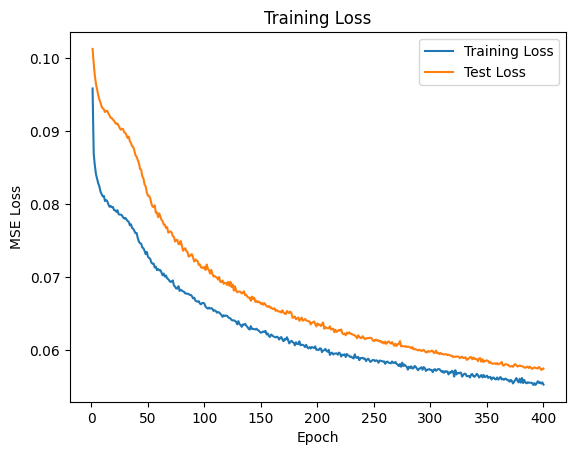
\includegraphics[width=\linewidth]{images/part1/training_bc.png}\\
      {\scriptsize Train/test loss — stopped early}
    \end{column}
  \end{columns}
\end{frame}

\begin{frame}{2. Diffusion models — background}
  \textbf{Forward (noising):}
  \[ x_t = \sqrt{\bar\alpha_t}\,x_0 + \sqrt{1-\bar\alpha_t}\,\epsilon,\qquad \epsilon\sim\mathcal{N}(0,I) \]
  \textbf{Reverse (denoising):} a network $\epsilon_\theta(x_t,t,c)$ predicts the added noise.
  \begin{columns}[T]
    \begin{column}{0.5\textwidth}
      \textbf{Training} ($\epsilon$-MSE)
      \begin{itemize}
        \item Sample $t$, add noise to get $x_t$
        \item Minimise $\lVert \epsilon_\theta(x_t,t,c)-\epsilon\rVert_2^2$
      \end{itemize}
    \end{column}
    \begin{column}{0.5\textwidth}
      \textbf{Sampling (control time)}
      \begin{itemize}
        \item Start from pure noise, iterate $T\!\to\!1$
        \item \alert{Deterministic}: drop ancestral noise $\Rightarrow$ posterior mean, low variance
      \end{itemize}
    \end{column}
  \end{columns}
  \vfill
  {\footnotesize Formulation follows \emph{Understanding Deep Learning} (Prince, 2023).}
\end{frame}

\begin{frame}{2. DDPM sampler — double pendulum}
  Sample an action chunk by \alert{ancestral denoising} (DDPM): start from pure noise $a_T\!\sim\!\mathcal{N}(0,I)$ and iterate $t:T\!\to\!1$ with $T=20$.
  \begin{columns}[T]
    \begin{column}{0.56\textwidth}
      \textbf{One reverse step}
      \[
        a_{t-1}=\tfrac{1}{\sqrt{1-\beta_t}}\!\Big(a_t-\tfrac{\beta_t}{\sqrt{1-\bar\alpha_t}}\,\epsilon_\theta(a_t,t,c)\Big)+\sqrt{\beta_t}\,z
      \]
      \begin{itemize}
        \item Linear $\beta$-schedule ($10^{-4}\!\to\!0.02$), EMA $0.999$
        \item \emph{Markovian}: every step removes a little noise, re-adds a little ($z\!\sim\!\mathcal{N}(0,I)$)
      \end{itemize}
    \end{column}
    \begin{column}{0.44\textwidth}
      \begin{alertblock}{Control tweak: drop $z$}
        Set ancestral noise $z=0\Rightarrow$ posterior mean each step. Low action variance is what lets it \emph{hold} the unstable upright — stray torque noise topples the pendulum.
      \end{alertblock}
      {\footnotesize All $T=20$ steps run every re-plan ($n_{\text{exec}}{=}1$).}
    \end{column}
  \end{columns}
\end{frame}

\begin{frame}{2. DDPM in action — noising \& denoising a chunk}
  \centering
  \includegraphics[width=\linewidth,height=0.74\textheight,keepaspectratio]%
    {images/part1/noising_denoising_overlay.png}\\
  {\scriptsize One mid-rollout expert chunk ($H{=}10$, two torques $u_1,u_2$). \textbf{Top:} forward process buries the expert (dashed) in noise; \textbf{bottom:} the deterministic reverse process recovers it almost exactly (cyan $\approx$ dashed, reconstruction MSE $\sim\!10^{-6}$).}
\end{frame}

\begin{frame}{3. Generating the expert dataset}
  Classical optimal-control pipeline — every sample dynamically valid by construction.
  \begin{enumerate}
    \item \textbf{Dynamics model} — planar 2-link EoM, all parameters read from \texttt{dp.xml}; smooth $\tanh$ friction (differentiable).
    \item \textbf{Trajectory optimisation} — direct collocation NLP solved with IPOPT (JAX autodiff); swing $[0,0,0,0]\to[\pi,0,0,0]$.
    \item \textbf{TVLQR tracking} — $u_t = u^\ast_t - K_t(x_t-x^\ast_t)$; nearest-neighbour re-lock for recovery.
    \item \textbf{Closed-loop rollout} in MuJoCo @ 20\,Hz, logging (state, torque).
  \end{enumerate}
  \begin{alertblock}{DAgger-style coverage}
    Perturb \emph{applied} torque ($\sigma=0.15\tau_{\max}$), log the \emph{clean} command $\Rightarrow$ teaches recovery from off-nominal states. Keep only successful rollouts ($\sim$600 trajectories).
  \end{alertblock}
\end{frame}

\begin{frame}{4. Diffusion Policy model (Chi et al.\ 2023)}
  Denoise an action chunk $a^{1:H}$ ($H=10$), conditioned on a clean context $c$.
  \begin{columns}[T]
    \begin{column}{0.54\textwidth}
      \textbf{Representation}
      \begin{itemize}
        \item Wrap safe angular features $\phi$
        \item Min--max normalise to $[-1,1]$ actions and velocities (stats saved)
        \item $c=$ last $K{=}4$ states $+$ goal $\in\mathbb{R}^{30}$
      \end{itemize}
      \textbf{Network} $\epsilon_\theta$
      \begin{itemize}
        \item \alert{Trajectory Transformer} (default) vs.\ MLP
        \item Linear $\beta$-schedule, $T=20$ steps, EMA $0.999$
      \end{itemize}
    \end{column}
    \begin{column}{0.46\textwidth}
      \begin{alertblock}{What makes the loop stable}
        \begin{itemize}
          \item Deterministic (noise-free) sampling
          \item \textbf{Single-step execution} ($n_{\text{exec}}{=}1$): re-plan every step
        \end{itemize}
      \end{alertblock}
      {\footnotesize Goal token is effectively constant (one upright goal) $\Rightarrow$ not truly conditionable.}
    \end{column}
  \end{columns}
\end{frame}

% ── Denoiser architectures ──────────────────────────────────────────────────
\begin{frame}{4. Denoiser networks — Transformer vs.\ MLP}
  \begin{columns}[c]
    \begin{column}{0.6\textwidth}
      \centering
      \includegraphics[width=\linewidth,height=0.78\textheight,keepaspectratio]%
        {images/part1/architecture/diffusion_transformer_architecture.png}\\
      {\scriptsize Trajectory \alert{Transformer} denoiser $\epsilon_\theta$ (default).}
    \end{column}
    \begin{column}{0.4\textwidth}
      \centering
      \includegraphics[width=\linewidth,height=0.78\textheight,keepaspectratio]%
        {images/part1/architecture/diffusion_mlp_architecture.png}\\
      {\scriptsize \alert{MLP} denoiser (ablation baseline).}
    \end{column}
  \end{columns}
\end{frame}

\begin{frame}{4. Trajectory Transformer denoiser}
  \centering
  \includegraphics[width=\linewidth,height=0.78\textheight,keepaspectratio]%
    {images/part1/architecture/diffusion_transformer_architecture.png}\\
  {\scriptsize Tokens: diffusion timestep \texttt{t} $+$ conditioning \texttt{c} $+$ action-chunk \texttt{a1\dots a10}, mixed by self-attention.}
\end{frame}

\begin{frame}{Attention heads — early vs.\ late denoising}
  \begin{columns}[c]
    \begin{column}{0.5\textwidth}
      \centering
      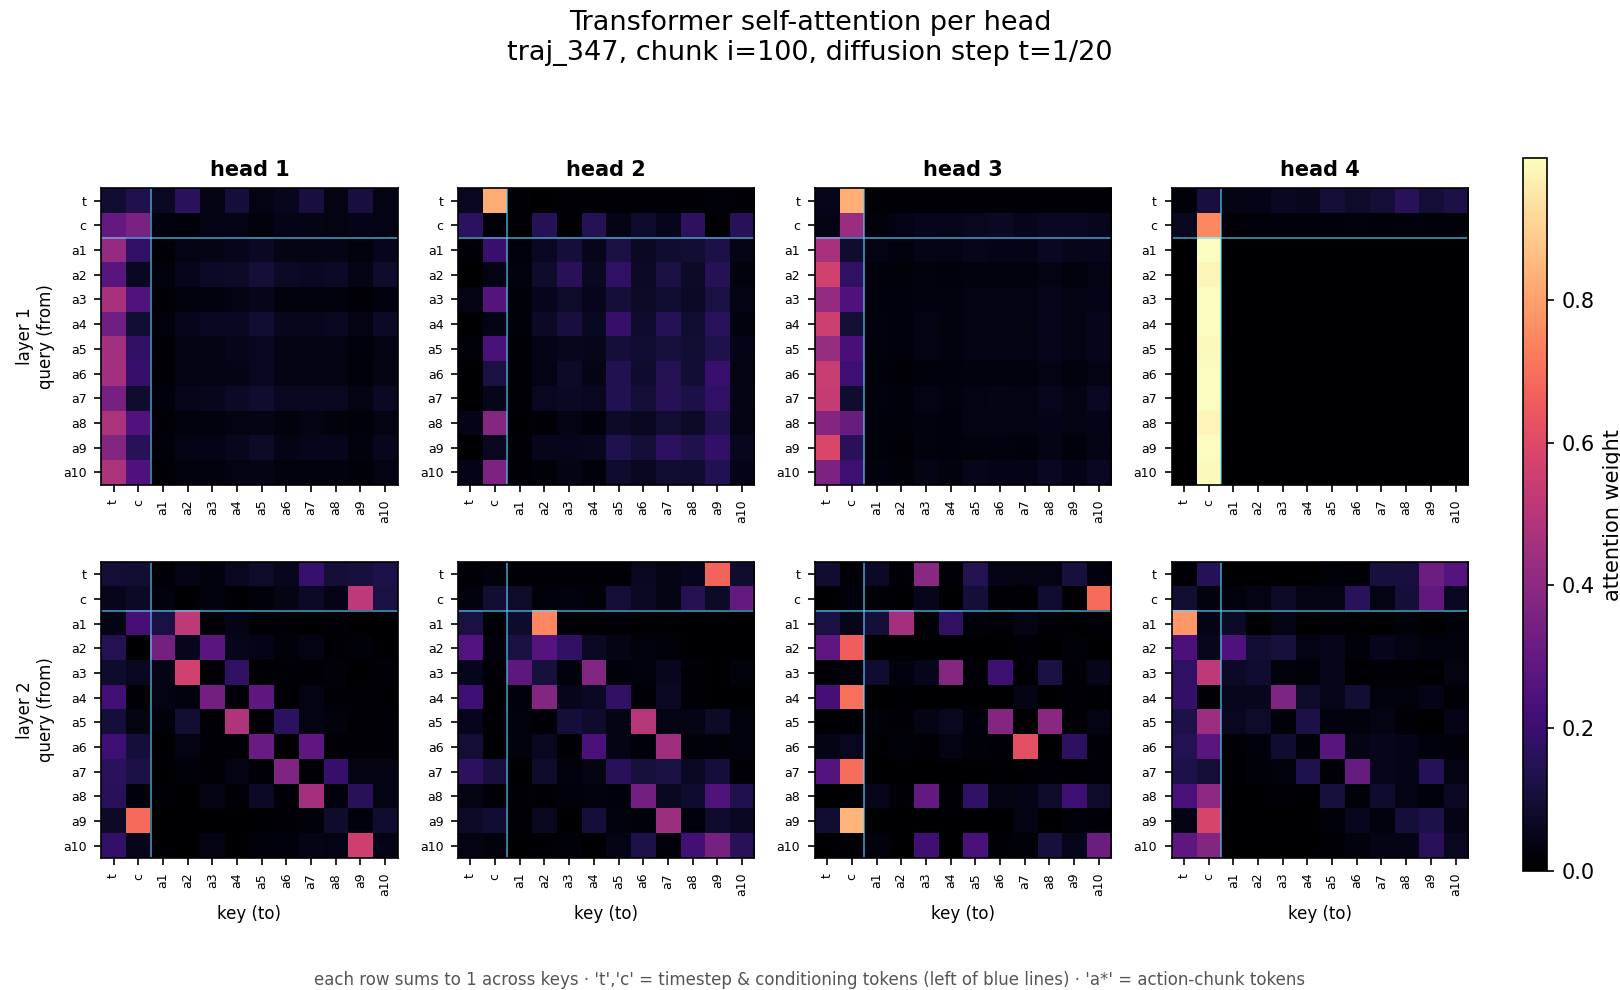
\includegraphics[width=\linewidth]{images/part1/architecture/attention_heads_start.png}\\
      {\scriptsize Early denoising ($t{=}1/20$): action tokens still attend to each other.}
    \end{column}
    \begin{column}{0.5\textwidth}
      \centering
      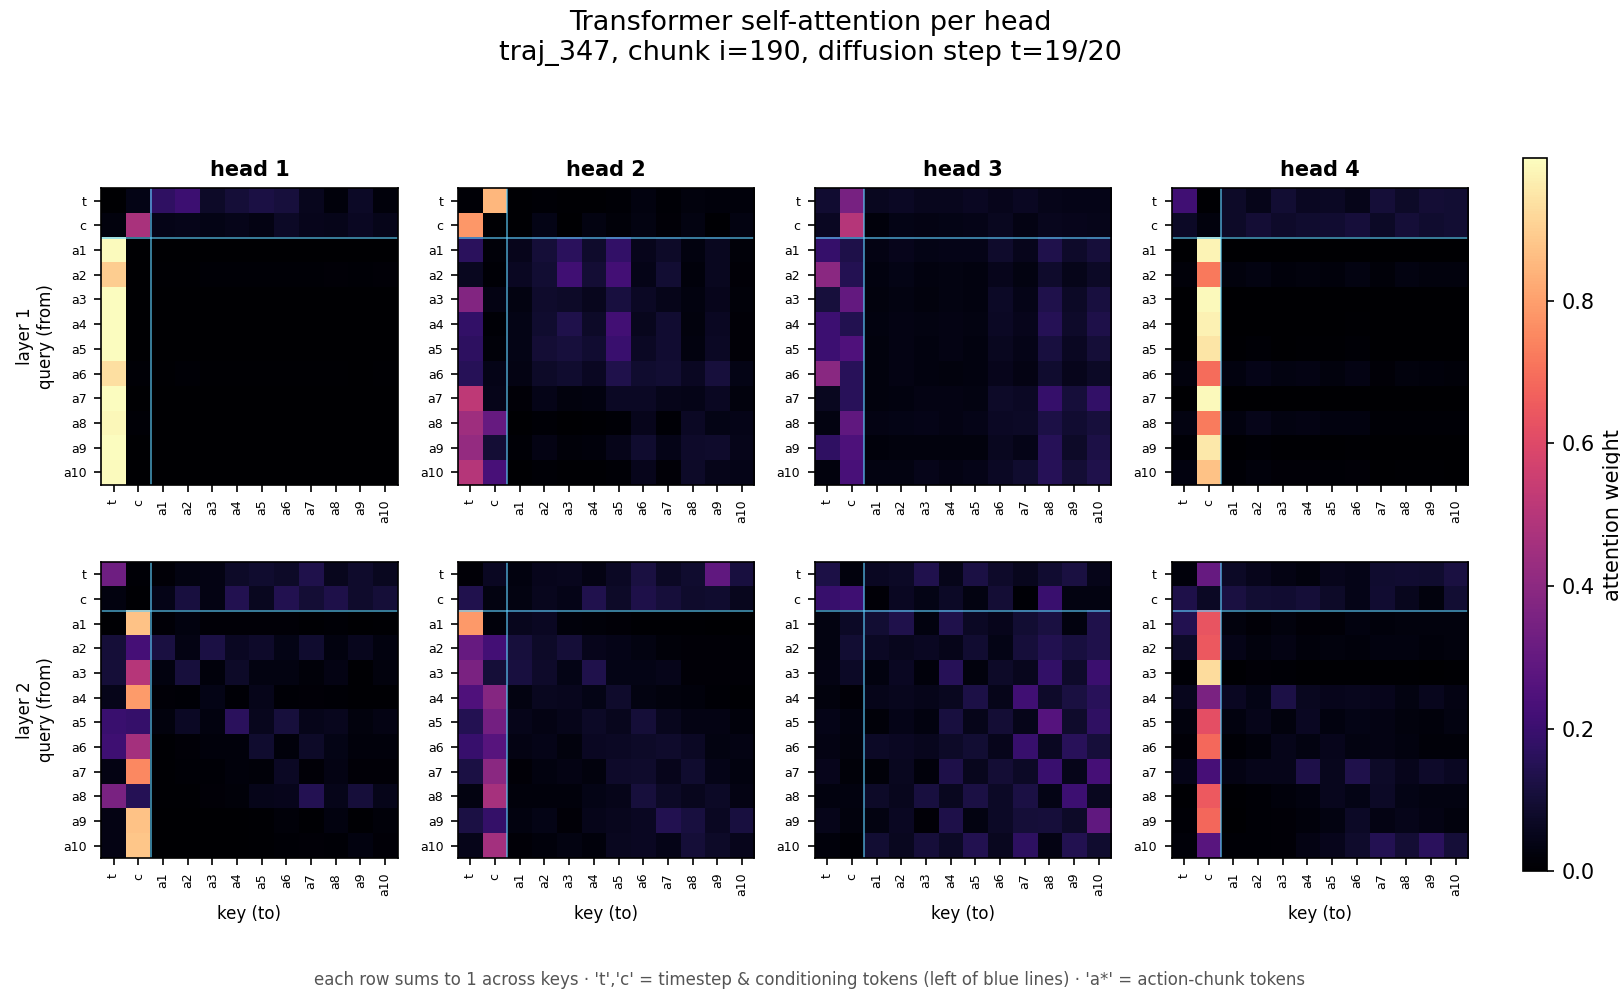
\includegraphics[width=\linewidth]{images/part1/architecture/attention_heads_fin.png}\\
      {\scriptsize Late denoising ($t{=}19/20$): mass collapses onto the \texttt{c} (conditioning) column.}
    \end{column}
  \end{columns}
  \vfill
  {\footnotesize\centering Rows sum to 1; \texttt{t,c} = timestep \& conditioning tokens (left of blue lines), \texttt{a*} = action-chunk tokens.\par}
\end{frame}

\begin{frame}{5. Comparison — aggregate metrics}
  \begin{columns}[T]
    \begin{column}{0.58\textwidth}
      \centering
      
\includegraphics[width=\linewidth]{images/part1/plots_comp_bc_diffusion/metrics_comparison.png}
    \end{column}
    \begin{column}{0.42\textwidth}
      Both swing up: \BC{} $100\%$, \DP{} $90\%$ (random init).
      \begin{itemize}
        \item \DP{} swings up \emph{faster} (5.07 vs 6.33 s) and lower IAE ($\sim$40\%)
        \item \BC{} holds upright far smoother ($8\times$ less $|\Delta u|$)
        \item \BC{} $\sim$28$\times$ cheaper per step (0.27 vs 7.6 ms)
      \end{itemize}
    \end{column}
  \end{columns}
\end{frame}

\begin{frame}{5. Comparison — robustness \& ablations}
  \begin{columns}[T]
    \begin{column}{0.33\textwidth}
      \centering
      
\includegraphics[width=0.92\linewidth]{images/part1/plots_comp_bc_diffusion/robustness_vs_noise.png}\\
      {\scriptsize \BC{} degrades more gracefully under observation noise.}
    \end{column}
    \begin{column}{0.33\textwidth}
      \centering
      
\includegraphics[width=0.92\linewidth]{images/part1/plots_compare_diffusion_exec_steps/nexec_sweep_success_rate.png}\\
      {\scriptsize Committing to $>1$ open-loop action destroys performance.}
    \end{column}
    \begin{column}{0.33\textwidth}
      \centering
      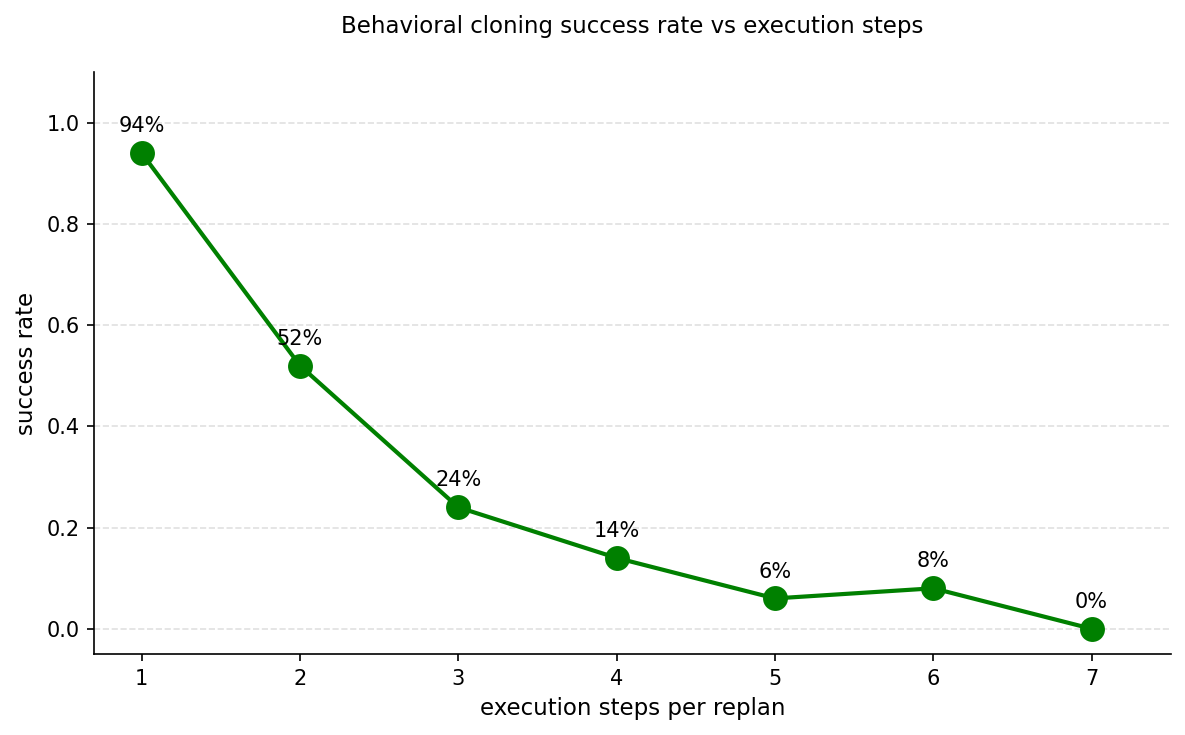
\includegraphics[width=0.92\linewidth]{images/part1/chart.png}\\
      {\scriptsize BC also performs best when open-loop actions are less than 1.}
    \end{column}
    
  \end{columns}
  \vfill
  \alert{Design choices are not free parameters:} transformer backbone (MLP collapses to $2\%$) and $n_{\text{exec}}=1$ are the difference between a working and a broken controller.
\end{frame}

\begin{frame}{Part I — takeaway}
  \begin{block}{On the double pendulum, \BC{} is the better controller}
    Both succeed, but BC holds the upright smoother, is more noise-robust, and
    $\sim$28$\times$ cheaper. The diffusion policy is fragile (needs per-step replanning,
    chatters near the unstable equilibrium).
  \end{block}
  Diffusion's edge — multimodal, temporally-correlated actions — does not pay off on a
  single, unimodal balance task.
\end{frame}

% ══════════════════════════════════════════════════════════════════════════════
\section{Part II — Robotic Cube Stacking}

\begin{frame}{Task \& control setup}
  Franka Emika Panda (7\,DoF) in MuJoCo / robosuite, task-space OSC\_POSE control.
  \begin{columns}[T]
    \begin{column}{0.5\textwidth}
      \textbf{Action space (7-D)}
      \begin{itemize}
        \item Translation $\Delta x,\Delta y,\Delta z$
        \item Rotation delta (axis-angle)
        \item Gripper state $\in[-1,1]$
      \end{itemize}
    \end{column}
    \begin{column}{0.5\textwidth}
      \textbf{State space}
      \begin{itemize}
        \item Stack: \textbf{32-D} (2 cubes)
        \item StackThree: \textbf{48-D} (3 cubes)
        \item cube poses, gripper-cube vectors, eef pose
      \end{itemize}
    \end{column}
  \end{columns}
  \vfill
  Goal: learn $\pi(a_{t:t+H}\mid s_t)$, receding-horizon control ($H$-step chunks).
\end{frame}

\begin{frame}{Dataset — MimicGen}
  \begin{itemize}
    \item Source: $\sim$10 human demos per task $\to$ MimicGen auto-generates large datasets ($D_0,D_1,\dots$).
    \item Four datasets used: \texttt{stack\_d0/d1}, \texttt{stack\_three\_d0/d1} — 1000 trajectories each.
    \item HDF5 / robomimic format; only state-relevant keys used (no images).
    \item A few source expert demonstration were used to generate new and create a complete dataset.
  \end{itemize}
  \begin{block}{Why it matters}
    Demonstrations contain \emph{several valid ways} to finish a stack $\Rightarrow$ a multimodal
    action distribution — the reason where diffusion is expected to perform better.
  \end{block}
\end{frame}

\begin{frame}{Models}
  \begin{columns}[T]
    \begin{column}{0.5\textwidth}
      \textbf{\BC{} baseline (MLP)}
      \begin{itemize}
        \item 5 linear layers ($256\to512$), LayerNorm, ReLU, dropout $0.1$
        \item State $\to 56$ values $\to (8,7)$ horizon
        \item MSE loss, Adam $10^{-3}$, 50 epochs
      \end{itemize}
    \end{column}
    \begin{column}{0.5\textwidth}
      \textbf{\DP{} Policy (Transformer)}
      \begin{itemize}
        \item \texttt{TransformerDenoiser}: 4 layers, $d{=}256$, 4 heads
        \item State + timestep tokens prepended to $H{=}8$ action tokens
        \item $\epsilon$-MSE, AdamW, $K{=}100$ steps, EMA $0.995$
      \end{itemize}
    \end{column}
  \end{columns}
  \vfill
  \textbf{Testing:} 50 episodes per model/task, control @ 20\,Hz, horizon 500 steps; success = cubes stacked.
\end{frame}


\begin{frame}{Evaluation — metrics \& results}
  Metrics per planning step: trajectory \textbf{jitter} $J$, \textbf{path effort} $E$, \textbf{joint cost} $C$; plus \textbf{success rate}.
  \begin{table}\centering\small
    \begin{tabular}{@{}llcc@{}}
      \toprule
      Task & Best success & \BC{} & \DP{} \\
      \midrule
      Stack       & ($H{=}8$/$4$) & $93\%$ & $\mathbf{98\text{--}100\%}$ \\
      StackThree  & ($H{=}8$)     & $56\%$ & $\mathbf{70\%}$ \\
      \midrule
      Replan @ $H{=}2$ (StackThree) & & $1\%$ & $\mathbf{36\%}$ \\
      Jitter ($H{=}8$, Stack)       & & $\mathbf{0.007}$ & $0.022$ \\
      \bottomrule
    \end{tabular}
  \end{table}
  \begin{itemize}
    \item \DP{} stacks more reliably and tolerates more frequent replanning.
    \item \BC{} is smoother (lower jitter) but completes fewer stacks — blurs the multiple valid motions.
    \item Both need the long $H{=}8$ horizon; $H{=}1$ breaks temporal coherence.
  \end{itemize}
\end{frame}

\begin{frame}{Evaluation — cube stacking results}
  \centering
  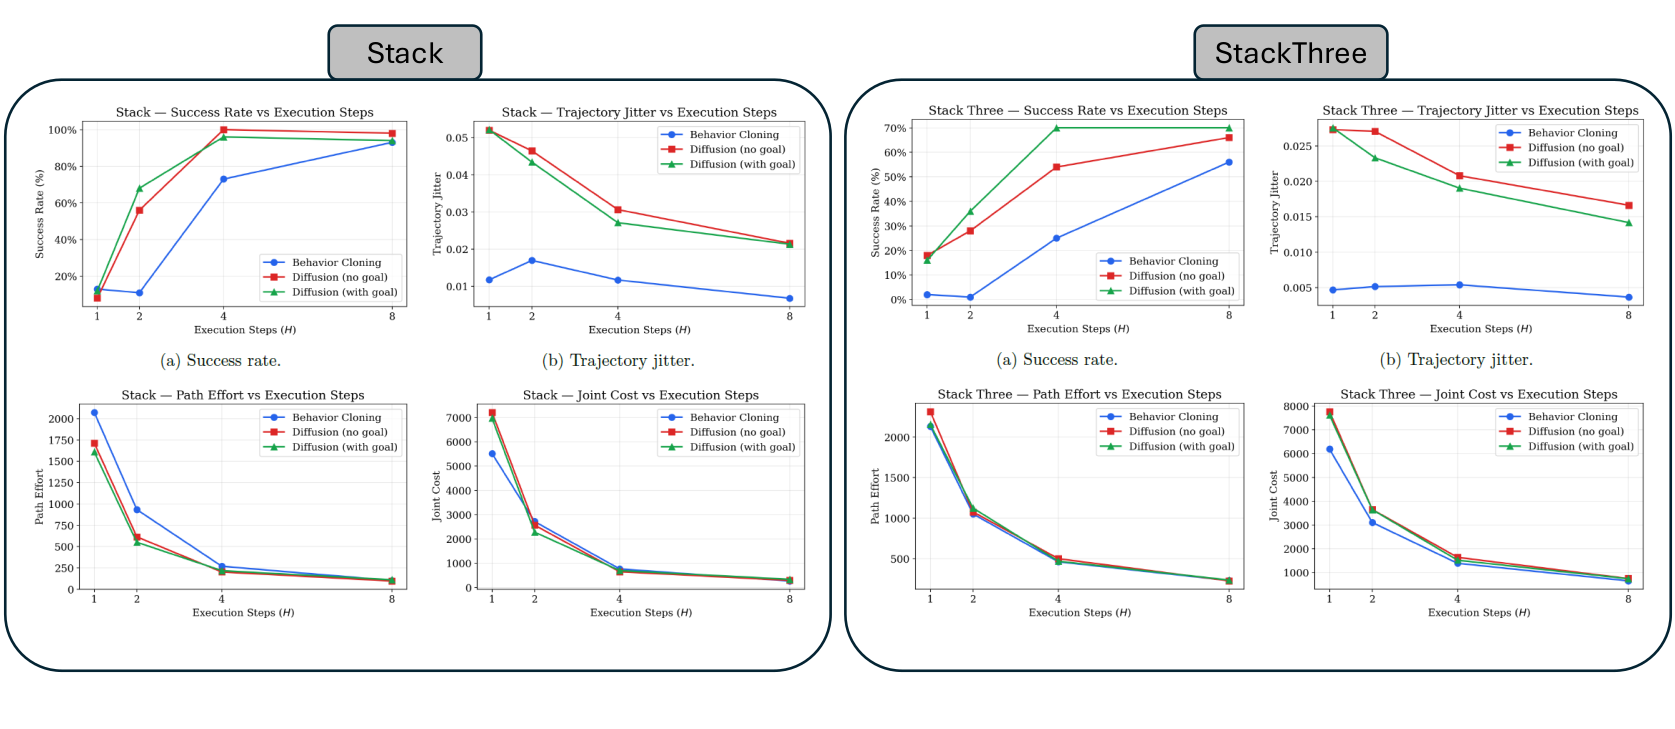
\includegraphics[width=\linewidth,height=0.8\textheight,keepaspectratio]{images/part2/cube_stack_results_figure.png}
\end{frame}

% ══════════════════════════════════════════════════════════════════════════════
\section{Conclusion}

\begin{frame}{Conclusion}
  \begin{block}{Neither method wins everywhere}
    The two tasks need \emph{opposite} replanning rates, and each method suits one.
  \end{block}
  \begin{columns}[T]
    \begin{column}{0.5\textwidth}
      \textbf{Double pendulum} \\ (fast, unstable, replan every step)
      \begin{itemize}
        \item \BC{} wins: smoother, robust, cheap
        \item Diffusion fragile, chatters
      \end{itemize}
    \end{column}
    \begin{column}{0.5\textwidth}
      \textbf{Cube stacking} \\ (multimodal, long horizon)
      \begin{itemize}
        \item \DP{} wins: higher success
        \item BC averages valid motions $\to$ fails more
      \end{itemize}
    \end{column}
  \end{columns}
  \vfill
  \centering\alert{BC: simple, cheap control of small balance tasks. \\ Diffusion: larger, multimodal manipulation.}
\end{frame}

\begin{frame}[standout]
  Thank you \\[1em]
  {\normalsize Questions?}
\end{frame}

\end{document}
